% Figure 1 for the Computational Linguistics short paper.
%
% A reconfiguration of reports/figures/commoncrawl_pipeline/commoncrawl_collection_pipeline.tex
% for this paper specifically. Two changes:
%
%   1. The two-track design is gone. The dissertation's figure emitted a "trend product" of
%      fixed-effort annual samples for frequency estimation alongside the corpus product.
%      This paper does not report salience, so that branch is dead weight; the pipeline now
%      terminates in the single quality-gated analysis corpus the semantic measures use.
%   2. Set in Palatino to match the journal body font, and laid out three column-groups over
%      a bottom row so it reads at roughly 1.9:1 rather than 3.5:1 and stays legible at the
%      32pc measure.
%
% The WET-first/WARC-second structure -- the part that actually makes web-scale diachronic
% collection affordable -- is unchanged.
%
% Build:
%   pdflatex -output-directory=reports/figures/cl scripts/cl_paper/fig1_pipeline_cl.tex

\documentclass[tikz,border=4pt]{standalone}

\usepackage[T1]{fontenc}
\usepackage[utf8]{inputenc}
\usepackage{palatino}
\usepackage{xcolor}
\usepackage{tikz}
\usetikzlibrary{arrows.meta,positioning,fit,backgrounds,calc}

\definecolor{wetblue}{HTML}{E8F1FA}
\definecolor{warcyellow}{HTML}{FFF4D8}
\definecolor{qualitygreen}{HTML}{EAF4EA}
\definecolor{outputgray}{HTML}{F2F2F2}
\definecolor{ink}{HTML}{222222}

\tikzset{
  stage/.style={
    rectangle,
    rounded corners=2.5pt,
    draw=ink!75,
    line width=0.45pt,
    align=center,
    text width=3.25cm,
    minimum height=1.05cm,
    inner sep=4.5pt,
    fill=white
  },
  wetstage/.style={stage, fill=wetblue},
  warcstage/.style={stage, fill=warcyellow},
  qualitystage/.style={stage, fill=qualitygreen},
  product/.style={stage, fill=outputgray, text width=3.6cm},
  group/.style={
    draw=ink!30,
    rounded corners=4pt,
    line width=0.5pt,
    inner sep=7pt,
    fill=black!2
  },
  group label/.style={
    font=\bfseries\footnotesize,
    text=ink!85,
    fill=white,
    inner sep=1.5pt
  },
  flow/.style={
    -{Stealth[length=2.0mm,width=1.7mm]},
    draw=ink!70,
    line width=0.55pt
  }
}

\begin{document}
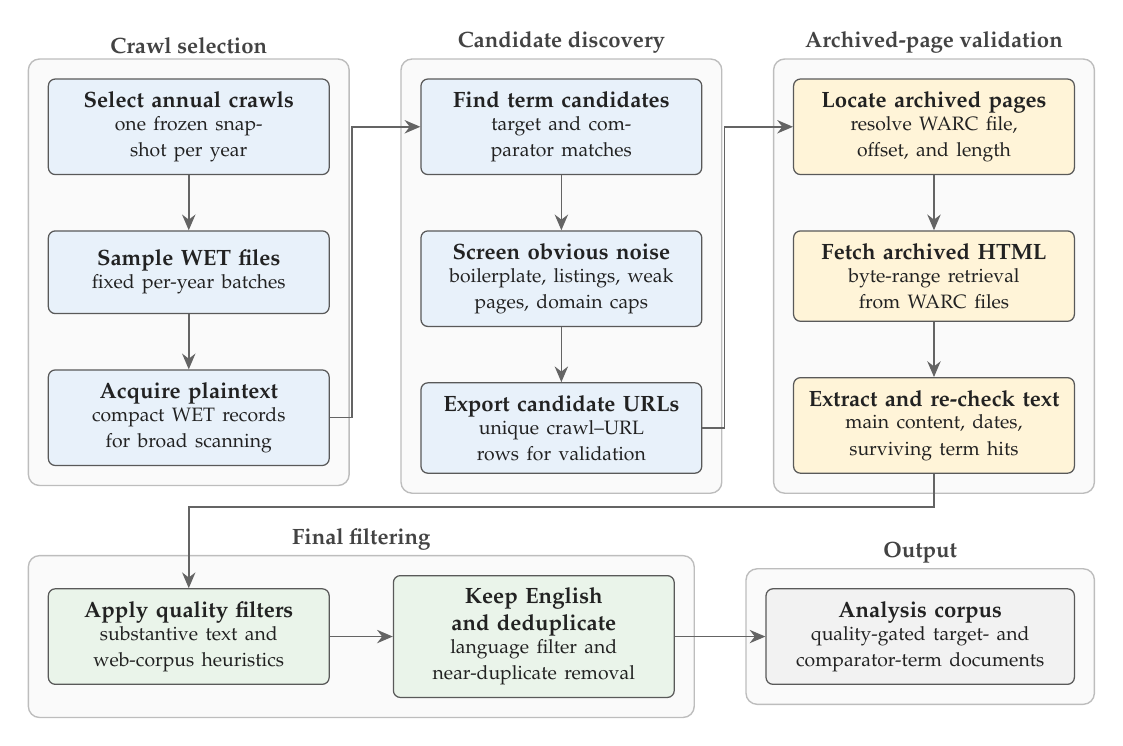
\begin{tikzpicture}[
  font=\footnotesize,
  node distance=0.70cm and 0.80cm,
  every node/.style={text=ink}
]

% ---- Column 1: crawl frame and WET acquisition ----
\node[wetstage] (crawl) {
  \textbf{Select annual crawls}\\[-0.15em]
  {\scriptsize one frozen snapshot per year}
};
\node[wetstage, below=of crawl] (sample) {
  \textbf{Sample WET files}\\[-0.15em]
  {\scriptsize fixed per-year batches}
};
\node[wetstage, below=of sample] (download) {
  \textbf{Acquire plaintext}\\[-0.15em]
  {\scriptsize compact WET records for broad scanning}
};

% ---- Column 2: WET candidate discovery ----
\node[wetstage, right=1.15cm of crawl] (scan) {
  \textbf{Find term candidates}\\[-0.15em]
  {\scriptsize target and comparator matches}
};
\node[wetstage, below=of scan] (triage) {
  \textbf{Screen obvious noise}\\[-0.15em]
  {\scriptsize boilerplate, listings, weak pages, domain caps}
};
\node[wetstage, below=of triage] (urls) {
  \textbf{Export candidate URLs}\\[-0.15em]
  {\scriptsize unique crawl--URL rows for validation}
};

% ---- Column 3: WARC validation and enrichment ----
\node[warcstage, right=1.15cm of scan] (resolve) {
  \textbf{Locate archived pages}\\[-0.15em]
  {\scriptsize resolve WARC file, offset, and length}
};
\node[warcstage, below=of resolve] (fetch) {
  \textbf{Fetch archived HTML}\\[-0.15em]
  {\scriptsize byte-range retrieval from WARC files}
};
\node[warcstage, below=of fetch] (extract) {
  \textbf{Extract and re-check text}\\[-0.15em]
  {\scriptsize main content, dates, surviving term hits}
};

% ---- Bottom row: quality gate and the single analysis corpus ----
\node[qualitystage, below=1.55cm of download] (quality) {
  \textbf{Apply quality filters}\\[-0.15em]
  {\scriptsize substantive text and web-corpus heuristics}
};
\node[qualitystage, right=0.80cm of quality] (langdedup) {
  \textbf{Keep English and deduplicate}\\[-0.15em]
  {\scriptsize language filter and near-duplicate removal}
};
\node[product, right=1.15cm of langdedup] (corpus) {
  \textbf{Analysis corpus}\\[-0.15em]
  {\scriptsize quality-gated target- and comparator-term documents}
};

% ---- Flow ----
\draw[flow] (crawl) -- (sample);
\draw[flow] (sample) -- (download);
\draw[flow] (download.east) -- ++(0.28,0) |- (scan.west);

\draw[flow] (scan) -- (triage);
\draw[flow] (triage) -- (urls);
\draw[flow] (urls.east) -- ++(0.28,0) |- (resolve.west);

\draw[flow] (resolve) -- (fetch);
\draw[flow] (fetch) -- (extract);

% Wrap from the end of the top row down to the start of the bottom row.
\draw[flow] (extract.south) -- ++(0,-0.42) -| (quality.north);

\draw[flow] (quality) -- (langdedup);
\draw[flow] (langdedup) -- (corpus);

% ---- Stage grouping boxes ----
\begin{scope}[on background layer]
  \node[group, fit=(crawl) (sample) (download),
    label={[group label]above:Crawl selection}] {};
  \node[group, fit=(scan) (triage) (urls),
    label={[group label]above:Candidate discovery}] {};
  \node[group, fit=(resolve) (fetch) (extract),
    label={[group label]above:Archived-page validation}] {};
  \node[group, fit=(quality) (langdedup),
    label={[group label]above:Final filtering}] {};
  \node[group, fit=(corpus),
    label={[group label]above:Output}] {};
\end{scope}

\end{tikzpicture}
\end{document}
